\documentclass[tikz]{standalone}
\usetikzlibrary{positioning}

\begin{document}
\begin{tikzpicture}[node distance=1cm, every node/.style={rectangle, minimum width=2cm, minimum height=1cm}]

    % Deep Q Learning box
    \node (dql) [draw, rectangle, minimum width=5.5cm, minimum height=7cm] {};
    \node [below right=-0.2cm and 0cm of dql.north west, font=\large] {\textbf{Deep Q Learning}};
    \node (policy) [below right=1cm and 0.2cm of dql.north west] {Policy Network};
    \node (policy_img) [right=0.5cm of policy] {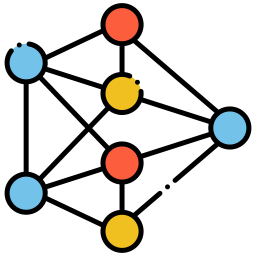
\includegraphics[width=1.5cm]{neural-network.png}};
    \node (target) [below=0.5cm of policy] {Target Network};
    \node (target_img) [right=0.5cm of target] {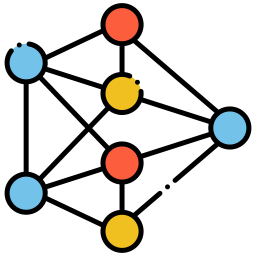
\includegraphics[width=1.5cm]{neural-network.png}};
    \node (buffer) [below=0.5cm of target] {Replay Buffer};
    \node (buffer_img) [right=0.5cm of buffer] {
\includegraphics[width=1.2cm]{buffer.png}};
    \node (env) [below=0.5cm of buffer] {Environment};
    \node (env_img) [right=0.5cm of env] {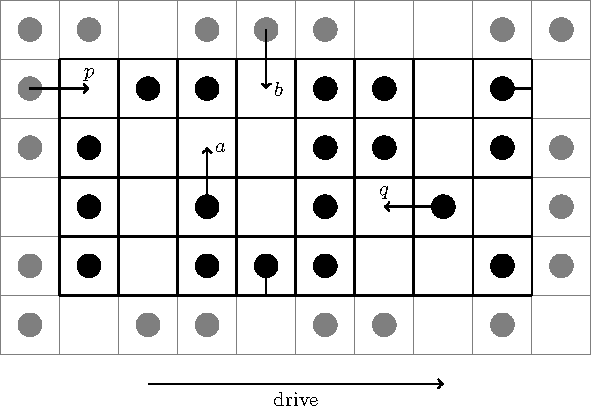
\includegraphics[width=2cm]{../..//Thesis/img/model/out/tasep_2d.pdf}};

\end{tikzpicture}
\end{document}